\begingroup
\let\cleardoublepage\clearpage
\tableofcontents
\endgroup

\addsec{О MIPT\LaTeX}

MIPT\LaTeX~"--- набор инструментов, стилей, макросов и~образцов, удобных для~написания работ на~русском языке студентами~Физтеха и~других вузов.
В~изначальной разработке и~апробации набора принимали участие аспиранты и~студенты кафедры микропроцессорных технологий Московского физико-технического университета:
\begin{itemize}
    \itemЮ.\,Байда
    \itemР.\,Фадеев
    \itemА.\,Леченко
    \itemП.\,Крюков
\end{itemize}

C~2015 года MIPT\LaTeX~"--- свободное программное обеспечение, распространяемое по~лицензии MIT.
Основной git-репозиторий доступен для~загрузки и~внесения изменений по~адресу \url{https://github.com/pavelkryukov/miptlatex}.

\pagebreak

\addsec{Рекомендуемые материалы для изучения \LaTeX}

\begin{enumerate}[label = \arabic*.]
    \itemЛьвовский С.\,М. \emph{\href{http://www.ihed.ras.ru/subsecond2007/papers/lv3ed.pdf}{Набор и вёрстка в системе \LaTeX}}~"--- 3-е изд. М.: МЦНМО, 2003.~"---448~c.
		\itemВоронцов К.\,В. \emph{\href{http://www.ccas.ru/voron/download/voron05latex.pdf}{\LaTeXe в примерах}}~"--- 2005.
\end{enumerate}

\addsec{Установка и настройка MiK\TeX}

MIPT\LaTeX{} предназначен для~работы с~дистрибутивом MiKTeX под ОС Windows.
Его можно загрузить с~официального сайта: \url{http://miktex.org/downloads}.
После установки нужно запустить программу \emph{MikTeX Options}~(рис.~\ref{fig:miktex}), чтобы~произвести настройку зеркала~(1) и~установку векторных шрифтов~(2).
Загрузка необходимых пакетов произойдёт автоматически при~первом запуске компилятора.

\begin{figure}[h]
    \centering
    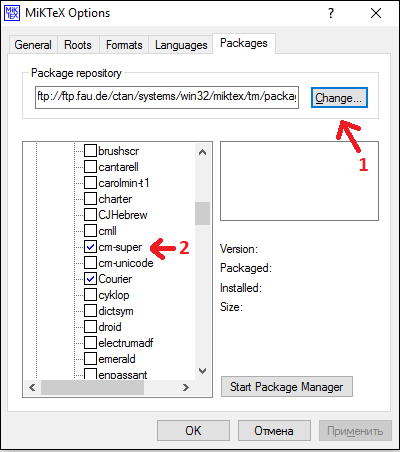
\includegraphics[scale = 1.0]{pictures/miktex.png}
    \caption{Интерфейс программы \emph{MikTeX Options}}
    \label{fig:miktex}
\end{figure}

\pagebreak

\addsec{Установка и настройка \TeX{}nicCenter}

\TeX{}nicCenter~"--- рекомендуемый нами для~работы на~Windows удобный редактор \TeX-файлов, который легко интегрировать как~с~MiK\TeX{}, так~и~с~внешними инструментами, .
Последняя версия редактора доступна для~загрузки на~официальном сайте: \url{http://www.texniccenter.org/download/}.

Чтобы создавать документы со списком литературы и алфавитным указателем на русском языке, необходимо произвести настройку препроцессора.
Для этого нужно запустить утилиту настройки профилей (\emph{Build/Define output profiles\ldots} или \emph{Alt+F7})~(рис.~\ref{fig:profiles}), нажать кнопку \emph{Import\dots} (1), выбрать файл конфигурации \emph{<workspace>/files/jobfile.tco} и~обновить пути к~файлам (2) директории~\emph{tools} на~актуальные.

\begin{figure}[h]
    \centering
    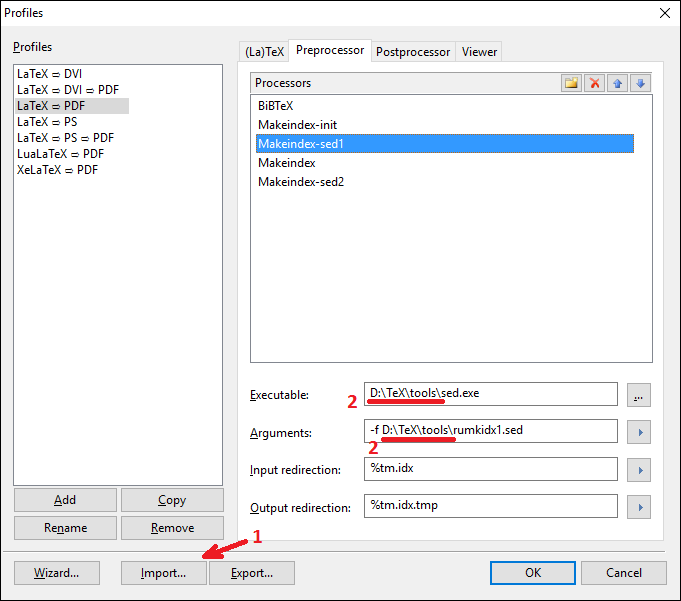
\includegraphics[scale = 0.7]{pictures/profiles.png}
    \caption{Интерфейс утилиты настройки профилей TeXnicCenter}
    \label{fig:profiles}
\end{figure}

\addsec{Рекомендуемая организация работы}

Установив и настроив инструменты, вы~можете создавать собственные документы с~использованием конфигурационных файлов MIPT\LaTeX.
Поскольку \LaTeX{} позволяет указывать относительные пути для~документов, то~удобно располагать документы в~поддиректориях рабочей копии git аналогично образцам работ; \eg \emph{<workspace>/works/masterthesis/} или~\emph{<workspace>/articles/ieee/}.
Подобная организация удобна для~коллективной разработки посредством git, так~как~одновременно позволяет разместить редактируемый документ в~системе контроля версий и~получать обновления MIPT\LaTeX.

Работающим в узкоспециализированных областях науки и~техники часто приходится ссылаться на~небольшое количество основополагающих статей, монографий или~диссертаций.
Чтобы избежать дублирования файлов, содержащих библиографическую информацию в~формате BiBTeX, рекомендуется сохранять её~в~едином файле (\eg \emph{<workspace>/global.bib}).
Подобный файл, наряду с~локальными изменениями конфигурационных файлом MIPT\LaTeX, может быть загружен на~ответвление основного репозитория MIPT\LaTeX.

\addsec{Образцы работ}

Практика показала, что наиболее простой и действенный способ вёрстки собственной работы заключается в изучении исходных файлов предшествующих работ.
Для этого в репозитории находятся 4 проекта, написанных с использованием MIPT\LaTeX:
\begin{enumerate}
    \item{About~"--- описание MIPT\LaTeX, которое вы сейчас читаете.}
    \item{Kraynov~"--- пример реферата по теоретической физике с большим количеством формул.}
    \item{VoIP~"--- пример реферата с иллюстрациями, перечислениями и разделённым списком литературы.}
\end{enumerate}

После проведения настройки настоятельно рекомендуется провести компиляцию всех трёх проектов, убедиться в~корректности вёрстки и~наличии списка литературы.

\addsec{Конфигурационные файлы}

\addsubsec{config.tex}

Файл config.tex содержит основные стилевые настройки документа для русской традиции и осуществляет подключение необходимых пакетов.

\addsubsec{macros.tex}

Файл macros.tex содержит определения наиболее употребительных макросов: сокращений, особых символов, специального форматирования, а также переопределения математических символов, свойственных русской традиции.

\addsubsec{paragraph.tex}

Подключение файла paragraph.tex запрещает разбивку параграфов между страницами~"--- в каких-то случаях это оказывается эстетичным.

\addsec{Пакеты}

\addsubsec{mips.sty}

Пакет mips.sty требуется для написания листингов на языке ассемблера архитектуры системы команд MIPS.

\addsec{Скрипты}

\addsubsec{trudy.bat}

Скрипт <<trudy.bat>> автоматически упаковывает работу для журнала <<Труды МФТИ>> в формат, требуемый редакцией.
\emph{раздел в разработке}

\addsubsec{endline}

Хорошим тоном написания документов в разметке \TeX считается размещение каждого предложения на отдельной строке.
Скрипт <<endline.pl>> проверяет соответствие указанного первым аргументом файла этой рекомендации.
В результате работы на экран выводятся номера строк файла, где эта рекомендация была нарушена.

Скрипт <<endline.sh>> запускает скрипт <<endline.pl>> для всех файлов *.tex, находящихся в указанной первым аргументом директории.

\addsubsec{nobr}

Как правило, при вёрстке текстов избегают появления так называемых <<висячих предлогов>>, \ie предлогов, находящихся на разных строках с последующим словом.
Аналогичные рекомендации действуют для коротких местоимений, таких как <<я>>, <<ты>>, <<он>>; а также частиц после основных слов (<<хотел~бы>>, <<думал~ли>>).
Скрипт <<nobr.pl>> заменяет <<обычные>> пробелы на <<неразрывные>> в большинстве требуемых случаев.
Аргументом входа является имя исходного файла, обработанный файл печатается на экран.

Скрипт <<nobr.sh>> проводит автоматическую замену необработанных файлов с расширением <<*.tex>> на обработанные в указанной директории.
Резервные копии файлов сохраняются в директории с расширением *.backup.

\emph{раздел в разработке}

\addsec{Создание списка литературы}

\addsec{Создание алфавитного указателя}

\addsec{Создание оглавлений}

